\documentclass[a4paper]{article}   % list options between brackets
\usepackage{CJK}
\usepackage{fullpage}
\usepackage{graphicx}
\usepackage{tabularx}
\usepackage{listings}
\usepackage{rotating}
\usepackage{setspace}
\usepackage{amsmath}
\usepackage{xcolor}
\usepackage{cite}

\lstset{numbers=left, numberstyle=\small, frame=shadowbox,
xleftmargin=2em,xrightmargin=2em, aboveskip=1em, breaklines,
extendedchars=false, tabsize=4, basicstyle=\linespread{1.0}\ttfamily,
commentstyle=\ttfamily\normal\small, keywordstyle=\color{blue!70}
}

% type user-defined commands here


\begin{document}
\begin{CJK}{UTF8}{gbsn}
\begin{spacing}{1.2}

\title{\vspace{120pt}\huge High Performance Computing\\ Homework 1\\[1em] \huge Understanding the Programming Platform\\[1em] \Large Report}
\author{\\[3em]\Large Peiyun Hu, 2010011297 \\ [1em]\Large Department of Computer Science \& Technology}
\date{Sep. 22, 2012}    % type date between braces
\maketitle

\section{Environment}             % section 1
\subsection{Hardware}

\subsubsection{CPU} \label{info:cpu}

Model Name: Intel(R) Core(TM)2 Quad CPU @ 2.93GHz\\
CPU MHz: 1600.000\\
Cores: 4\\
But actually, only one core is involved in this task. What is more, the '1600 MHz' means that at which the processor is running right now, and '2.93 GHz' is the maximum CPU Speed. 
\subsubsection{Memory} 
Total Memory: 4055940 KB

\subsubsection{Cache} \label{info:cache}
Cache Size: 4096 KB

%\subsubsection{Disk} 


\subsection{Software}     % subsection 1.1

\subsubsection{OS} 
Linux version 2.6.38-8-generic
\subsubsection{Compiler} 
gcc version 4.5.2 (Ubuntu/Linaro 4.5.2-8ubuntu4)
\subsubsection{Compiler Options}
Please refer to makefile.

\subsubsection{Timing Method}
As for the timing method, only meaningful calculation time are counted, which means that time spent in initialization and output are excluded from the final time. \\

Additionally, there are minute differences under different conditions. Firstly, in the vector-to-vector($\vec{a}, \vec{b}$) computation, one float operations are involved in each pair of elements, which is a multiplication of $a_i \times b_i$. Secondly, in the matrix-to-vector calculation, two float operations need to be counted in each pair, which is a multiplication and an addition. Besides, matrix-to-matrix condition is similar with the m2v's condition.\\

Consequently, assuming that the problem number of rows and columns are both n, we could infer that:\\

\begin{align}
\label{align:flops}
\text{FLOPS}_{v2v} = \frac{n}{t} \\
\text{FLOPS}_{m2v} = \frac{2n^2}{t} \\
\text{FLOPS}_{m2m} = \frac{2n^3}{t}
\end{align}

\section{Performance}
\subsection{Theoretical Peak Performance}
As is shown in \ref{info:cpu}, it is known that A Core 2 Quad has 4 cores. HPC world uses the following formulae for node theoretical peak performance:

\begin{center}
\bf
Node performance in GFLOPS = (CPU speed in GHz) x (number of CPU cores) x (CPU instruction per cycle) x (number of CPUs per node).\cite{plain:flops_formulae}
\end{center}

In this sequential task, the node performance is as below:
\begin{align}
\text {Performance }= 2.93 \text{GHz }\times 1 \times 4 \times 1 = 11.72 \text {GHz}
\end{align}
An important note about CPU instruction per cycle is 4, as is shown in \cite{plain:intel_manual}.

Moreover, considering there are two indicators of cpu speed, we choose the higher one, because the cpu is smart enough to gear up when more calculation is needed. So the indicator '2.93 GHz' is more appropriate.


\subsection{Experiment Results}

\subsubsection{Vector-Vector}
The efficiency in varied size of dataset is shown as Figure \ref{figs:flops_vv}.As we can see from the chart, in small dataset, the performance of float rivals that of double. Because the dataset is rather small that the time of timing is not short enough to be ignored, even timing possessed most of time consumed.\\

When dataset gets bigger, float is almost twice faster than double, owing to their length. 

\begin{figure}[htbp]
\centering
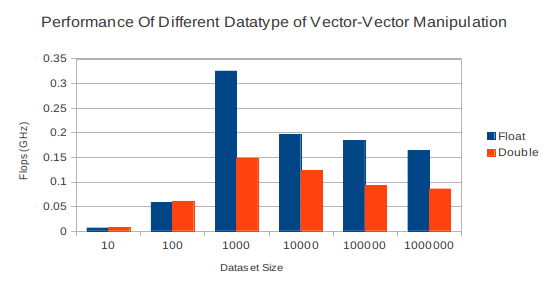
\includegraphics[width=12cm]{figs/vv.png}
\caption{Performance of Vector-Vector Manipulation With Different Implements}
\label{figs:flops_vv}
\end{figure}

\subsubsection{Matrix-Vector}
The efficiency in varied size of dataset is shown as Figure \ref{figs:eff_mv}. As shown in the chart, the efficiency of float calculation is rather stable. And the double is increasing gradually, but stay lower than float operation. 



\begin{figure}[htbp]
\centering
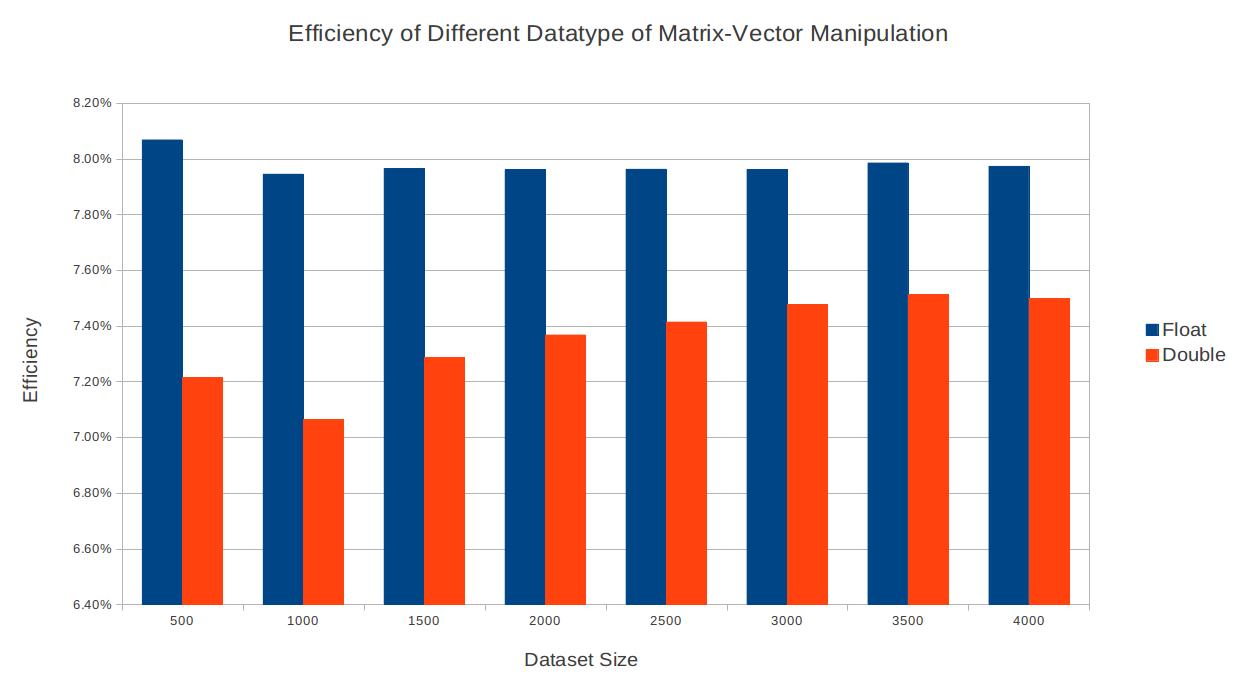
\includegraphics[width=12cm]{figs/eff_mv.png}
\caption{Efficiency of Matrix-Vector Manipulation With Different Implements}
\label{figs:eff_mv}
\end{figure}

\subsubsection{Matrix-Matrix}
The efficiency in varied size of dataset is shown as Figure \ref{figs:eff_mm}. Two methods of multiplication are involved. \\

The first one is simple and intuitive. After reading in the matrix, do the multiplicaiton directly like below:
\begin{lstlisting}[language=C]
for(i=0; i<a_rows; i++)
	for(j=0; j<b_cols; j++)
		for(k=0; k<a_cols; k++)
			res[i*a_cols+j] += v1[i*a_cols+k] * v2[k*b_cols+j];
\end{lstlisting}

But when considering taking advantage of cache, we can make it better by preprocessing the second matrix \textbf{$v_2$}. By transposing \textbf{$v_2$}, we can achieve a better hit rate when accessing \textbf{$v_2$}, owing to the linear arrangement of the array in the physical storage. And the code is a little different from above:

\begin{lstlisting}[language=C]
for(i=0; i<a_rows; i++)
	for(j=0; j<b_cols; j++)
		for(k=0; k<a_cols; k++)
			res[i][j] += v1[i*a_cols+k] * v2[j*a_cols + k];	
\end{lstlisting}

We can notice that the index of each array now increment by 1.And, we got almost 4 times faster than that of former method as is shown in \ref{figs:eff_mm}.

What is more \textbf{interesting} is, in Figure \ref{figs:eff_mm}, the float implement of first method is nearly on the same level with the second method. To interprete this, we should review \ref{info:cache}. The cache can hold:
\begin{align}
\frac{4096*1024}{500^2 * 2 * 4} = 2.097
\end{align}
32-bit single-precision floating numbers. That is to say, without the optimization of memory access, CPU could still reach a high hit rate. \\

But cache is not big enough to store double-precision floating matrixs of this size at one time. That is why we see a sharp contrast between performance of float and performance of double, in the first method. 

\begin{figure}[htbp]
\centering
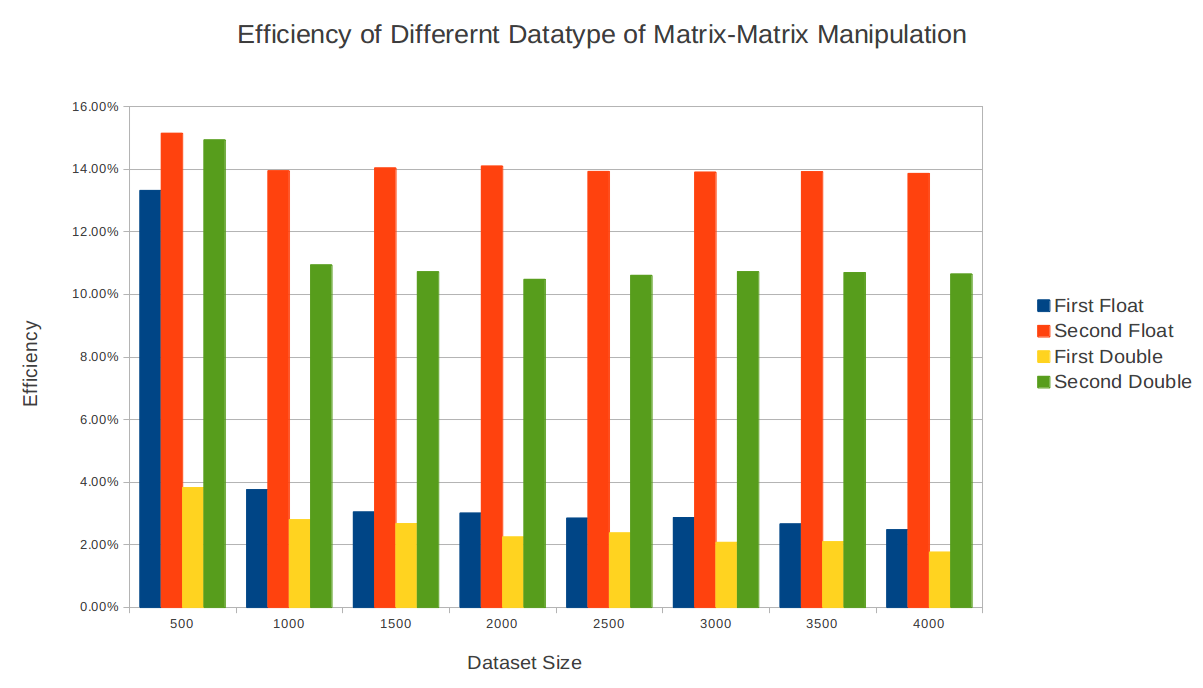
\includegraphics[width=12cm]{figs/eff_mm.png}
\caption{Efficiency of Matrix-Matrix Manipulation With Different Implements}
\label{figs:eff_mm}
\end{figure}

\section{Further Discussion}
Besides, noticing that SSE, which was firstly introduced in Pentium III, added eight new-bit registers known as XMM0 through XMM7, the cpu could handle 4 32-bit float at one time. Owing to SSE2 introduced later since Pentium Series, the usage of XMM is expanded to 64-bit double-precision mode. Additionally, the AMD64(originally called x86-64) added further eight registers from XMM8 to XMM15.

So with SSE programmed inline, we could further enhance the performance. However, it is a little embarassing in this task, for I did not find a easy way to mutiply using SSE. 

\bibliographystyle{plain}
\bibliography{bibitex}

\appendix
\section*{Appendix}
\section{Implement of Vector-Vector}
\begin{lstlisting}{language=[ANSI]C}

#include <stdio.h>
#include <stdlib.h>
#include <time.h>

#define start_time clock_gettime(CLOCK_MONOTONIC, &start);
#define end_time clock_gettime(CLOCK_MONOTONIC, &finish);

struct timespec start, finish;
	
int main(int argc, char *argv[]){
    int output_switch; 
    char *input_file_name;
    char *output_file_name;
    FILE* pfile;
    
    /* resolve the input arguments */
    if (argc < 2){
        printf("Error! the number of arguments is less(%d)!\n", argc);
        system("pause");
        return 0;
    }
    input_file_name = argv[1]; // get input file name

    output_switch = 0;     // output results or not 
    if (argc > 2) {       
        output_switch = 1;
        output_file_name = argv[2];
    }

    if ((pfile = fopen(input_file_name, "rb")) == NULL){
        printf("file: %s can not be opened \n", input_file_name);
        system("pause");
        return 0;
    }

    int size;
    float *v1, *v2, *res;

// set size
	fread((void*)(&size), sizeof(int), 1, pfile);

// alloc
	v1 = (float*)malloc(size * sizeof(float));
	v2 = (float*)malloc(size * sizeof(float));
	res = (float*)malloc(size * sizeof(float));

// read in data
	fread((void*)v1, sizeof(float), size, pfile);
	fread((void*)v2, sizeof(float), size, pfile);

// set start
	start_time

// calculate
	int i;
	for(i=0; i<size; i++)
		res[i] = v1[i] * v2[i];	

// set end
	end_time
	printf("%d %.16lf\n", size, finish.tv_sec-start.tv_sec + (double)(finish.tv_nsec - start.tv_nsec) / 1000000000.0);

#ifndef SILENT
    for (i = 0; i < a_rows; i ++){
        printf("%f ", v1[i]);
    }
    printf("\n");
#endif

    /* output results */ 
    if (output_switch){
        if ((pfile = fopen(output_file_name, "wb")) == NULL){
            printf("file: %s can not be opened \n", output_file_name);
            system("pause");
            return 0;
        }
        fwrite(res, sizeof(float), size, pfile);
        fclose(pfile);
    }
}
\end{lstlisting}

\section{Implement of Matrix-Vector}


\begin{lstlisting}{language=[ANSI]C}

#include <stdio.h>
#include <stdlib.h>
#include <time.h>
#include <memory.h>

#define start_time clock_gettime(CLOCK_MONOTONIC, &start);
#define end_time clock_gettime(CLOCK_MONOTONIC, &finish);

struct timespec start, finish;

int main(int argc, char *argv[]){
    int output_switch; 
    char *input_file_name;
    char *output_file_name;
    FILE* pfile;
    
    /* resolve the input arguments */
    if (argc < 2){
        printf("Error! the number of arguments is less(%d)!\n", argc);
        system("pause");
        return 0;
    }
    input_file_name = argv[1]; // get input file name

    output_switch = 0;     // output results or not 
    if (argc > 2) {       
        output_switch = 1;
        output_file_name = argv[2];
    }

    if ((pfile = fopen(input_file_name, "rb")) == NULL){
        printf("file: %s can not be opened \n", input_file_name);
        system("pause");
        return 0;
    }

    int a_rows, a_cols, b_cols;
    float *v1, *v2, *res;

// set size
    fread((void*)(&a_rows), sizeof(int), 1, pfile);
    fread((void*)(&a_cols), sizeof(int), 1, pfile);

// alloc
    v1 = (float*)malloc(a_rows*a_cols * sizeof(float));

    v2 = (float*)malloc(a_cols * sizeof(float));
    res = (float*)malloc(a_cols * sizeof(float));

// read in data
    fread((void*)v1, sizeof(float), a_rows*a_cols, pfile);
    fread((void*)v2, sizeof(float), a_cols, pfile);
// memset
    memset(res, 0.0, a_rows * sizeof(float));

// set start
    start_time

// calculate
    int i, j;
    for(i=0; i<a_rows; i++)
            for(j=0; j<a_cols; j++)
                    res[i] += v1[i*a_cols+j] * v2[j];

// set end
    end_time
    printf("%d %d %.16lf\n", a_rows, a_cols, finish.tv_sec-start.tv_sec + (float)(finish.tv_nsec - start.tv_nsec) / 1000000000.0);

    printf("a: %d %d \n", a_rows, a_cols);
#ifndef SILENT
    for (i = 0; i < a_rows; i ++){
        for (j = 0; j < a_cols; j ++) 
            printf("%f ", v1[i*a_cols+j]);
            printf("\n");
    }
#endif

    /* output results */ 
    if (output_switch){
        if ((pfile = fopen(output_file_name, "wb")) == NULL){
            printf("file: %s can not be opened \n", output_file_name);
            system("pause");
            return 0;
        }
        fwrite(res, sizeof(float), a_cols*b_cols, pfile);
        fclose(pfile);
    }
    
}
\end{lstlisting}

\section{Implement of Matrix-Matrix}

\begin{lstlisting}{language=[ANSI]C}

#include <stdio.h>
#include <stdlib.h>
#include <time.h>
#include <memory.h>

#define start_time clock_gettime(CLOCK_MONOTONIC, &start);
#define end_time clock_gettime(CLOCK_MONOTONIC, &finish);

struct timespec start, finish;

int main(int argc, char *argv[]){
    int output_switch; 
    char *input_file_name;
    char *output_file_name;
    FILE* pfile;
    
    /* resolve the input arguments */
    if (argc < 2){
        printf("Error! the number of arguments is less(%d)!\n", argc);
        system("pause");
        return 0;
    }
    input_file_name = argv[1]; // get input file name

    output_switch = 0;     // output results or not 
    if (argc > 2) {       
        output_switch = 1;
        output_file_name = argv[2];
    }

    if ((pfile = fopen(input_file_name, "rb")) == NULL){
        printf("file: %s can not be opened \n", input_file_name);
        system("pause");
        return 0;
    }

    float *v1, *v2, *res;
    int a_rows, a_cols, b_cols;

// set size
    fread((void*)(&a_rows), sizeof(int), 1, pfile);
    fread((void*)(&a_cols), sizeof(int), 1, pfile);
    fread((void*)(&b_cols), sizeof(int), 1, pfile);
// alloc
    v1 = (float*)malloc(a_rows* a_cols * sizeof(float));
    v2 = (float*)malloc(a_cols* b_cols* sizeof(float));
    res = (float*)malloc(a_rows*b_cols* sizeof(float));

// read in data
    fread((void*)v1, sizeof(float), a_rows*a_cols, pfile);
    fread((void*)v2, sizeof(float), a_cols*b_cols, pfile);

    fclose(pfile);
    
// memset
    memset(res, 0.0, a_rows * b_cols * sizeof(float));
// set start
    start_time

// calculate
    int i, j, k;
    for(i=0; i<a_rows; i++)
        for(j=0; j<b_cols; j++)
            for(k=0; k<a_cols; k++)
                res[i*a_cols+j] += v1[i*a_cols+k] * v2[k*b_cols+j];

// set end
    end_time
    printf("%d %d %d %.16lf\n", a_rows, a_cols, b_cols, finish.tv_sec-start.tv_sec + (double)(finish.tv_nsec - start.tv_nsec) / 1000000000.0);
   
    printf("a: %d %d \n", a_rows, a_cols);
    printf("b: %d %d \n", a_cols, b_cols);
    printf("c: %d %d \n", a_rows, b_cols);
#ifndef SILENT    
    for (i = 0; i < a_rows; i ++){
        for (j = 0; j < a_cols; j ++) 
            printf("%f ", v1[i*a_cols+j]);
            printf("\n");
    }
#endif 

    /* output results */ 
    if (output_switch){
        if ((pfile = fopen(output_file_name, "wb")) == NULL){
            printf("file: %s can not be opened \n", output_file_name);
            system("pause");
            return 0;
        }
        fwrite(res, sizeof(float), a_cols*b_cols, pfile);
        fclose(pfile);
    }
}
\end{lstlisting}


\end{spacing}
\end{CJK}
\end{document}
